\chapter{Introduction}
\label{chap:introduction}

%There have been few pivotal moments in history when science fiction became science fact and fundamentally reshaped the use of technology in our society\textcolor{blue}{/increased the impact of technology on society/opened a new technological frontier/brought technology to the next level/altered forever the way technology is perceived}. 

In 1966, Richard Fleischer directed \emph{Fantastic Voyage}, a film about the voyage of a miniaturized submarine used to cruise along human blood vessels and repair the damaged caused to the scientist's brain by a blood clot. The idea of treating from the inside damaged cells or organs fuelled the imagination of the next generation scientists and shaped the incipient field of nanomedicine. Less than 30 years later, science fiction became science fact and Doxil was approved by the US Food and Drug Administration in 1995 as the first nanodrug comercially available \citep{barenholz_doxil_2012}. Although 20 years after this milestone nano-submarines are still a long way off, nanomedicine is a well-established research field and dozens of products are under clinical trials or have been approved by the relevant health agencies.

The precursor to the nanomedicine breakthrough can be found in the tremendous progress in nanoparticles research observed in the 60s and 70s of the last century. Nanoparticles (NPs) are objects with \emph{one or more external dimensions in the size range from 1 nm to 100 nm} (European Commission Recommendation for nanomaterial (2011/696/EU)) and have a preeminent position in the continuously growing world of nanotechnology, employed as paints or cosmetic products \citep{guterres_polymeric_2007}. Besides, the applcation of NPs in the emerging field of nanomedicine opens up exciting prospects \citep{nie_nanotechnology_2007, sahoo_nanotech_2003, wickline_nanotechnology_2003, zhou_nano-enabled_2014, rosen_rise_2005}, especially considering their possibilities as platforms for drug-delivery \citep{wang_nanoparticle_2012} or encapsulating imaging agents \citep{tao_shape-specific_2011}.

The development of NPs is currently focused towards tailoring nanodrug carriers with flexible surface functionalisations and controlled morphologies \citep{euliss_imparting_2006,yang_shape-memory_2005}. The morphology of NPs is typically specified by parameters like size, shape, density or chemical composition of the particle, which are fundamental and defining aspects of the particle functions and determine their applicability in real-world medical applications \citep{vittaz_effect_1996}. In this regard, the size of NPs is one of the most crucial phsicochemical properties of nanodrugs, because it delimits whether they can intrude into the biological cells or the targeted tumor sites. An accurate and reliable description of the morphological traits of the NPs is therefore of vital importance for their favorable translation into successful nanomaterials.

%\begin{figure}[hbt]%[htbp]
%	\centering
%%%%%%	        \def\svgwidth{0.75\linewidth}
%		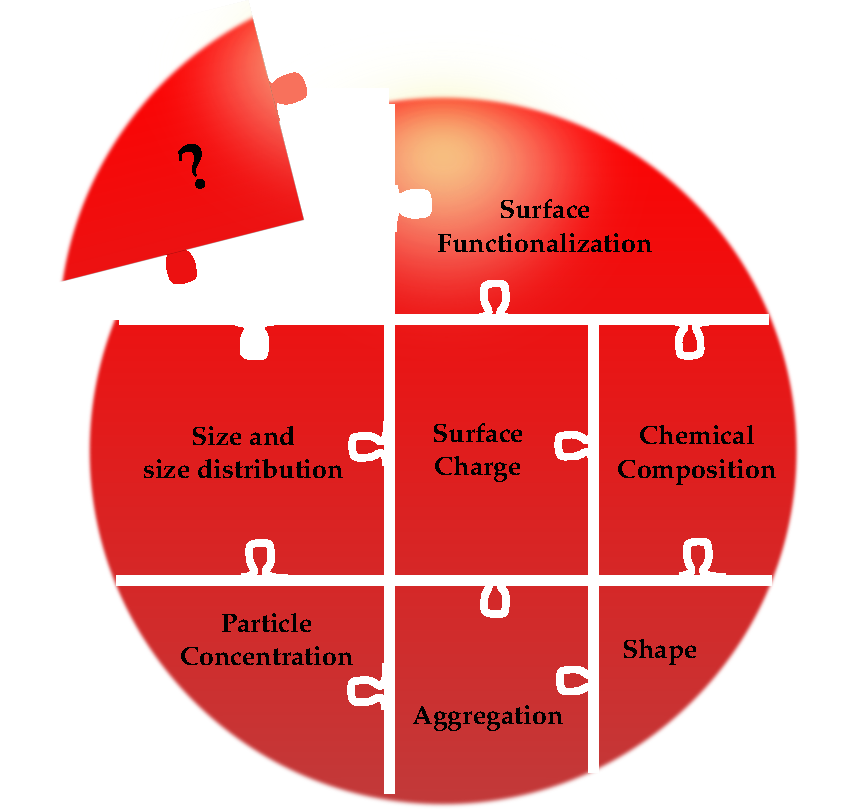
\includegraphics[width=0.65\textwidth]{Figures/NanoparticlesProperties.pdf}
%		\caption[Properties of nanoparticles]{Relevant properties of nanoparticles used in medical applications.}
%		\label{fig:NanoparticlesProperties}
%\end{figure}

The term \emph{nanometrology} refers to the science of accurate and correct measurement of relevant properties at the nanometre range. A central concept in metrology is \emph{traceability}, which refers to the ability of relating the measured value i.e. measurand to a base unit definition of the Internation System of Units (SI system) by an unbroken chain of comparisons with known uncertainties. This allows an objective comparison of the results obtained by different methods based on a consistent uncertainty budget associated to the measurand. The fundamental research in the field of metrology in Germany is addressed by its national metrology institute, the Physikalisch-Technische Bundesanstalt (PTB). Founded in 1887, the PTB is devoted among other metrological activities to the determination of fundamental and natural constants or the technology transfer with the industry.

In the nanoscale level, PTB is involved in the development of the dimensional nanometrology field, which studies the measurement of the physical size or distances of a given nanomaterial and traces it back to the \emph{nm} unit. There are several available techniques which are suitable for the sizing of NPs, though not all provide a traceable measurement. A prime example is dynamic light scattering (DLS), the most widely used tool in nanomedicine \citep{murphy_static_1997, hallett_vesicle_1991, egelhaaf_determination_1996, takahashi_precise_2008, jans_dynamic_2009, hoo_comparison_2008}. DLS is well-established and has indisputable advantages in the size characterization of the NPs, e.g. easy-to-use instrumentations, fast and low-cost operation, but it is not capable of a traceable size determination as there is no general relationship between the measured hydrodynamic diameter and the physical size of the NPs \citep{meli_traceable_2012}.

Other ensemble techniques extensively used are differential centrifugal sedimentation (DCS) \citep{fielding_correcting_2012} and Nanoparticle Tracking Analysis (NTA), both capable of measuring the NPs in suspension, i.e. in their native medium. While DCS is based on the sedimentation of NPs through a density gradient, NTA is a single-particle counting method that relates the Brownian movement of the particles with the measured laser light scattering. The particle size distribution obtained with DCS is traced down to a calibration standard of known size and density, resulting in a non-traceable measurement. Similarly to DLS, the NTA measurand derives from the hydrodynamic properties of the NPs \citep{varga_towards_2014}.

Microscopic tools are also frequently used for structural investigations \citep{joensson_morphology_1991,silverstein_microstructure_1989} and proved to be useful techniques for solid NPs due to their SI traceability achieved by coupling the measurement table with a laser interferometer \citep{meli_traceable_2012}. Nevertheless, techniques such as transmission scanning electron microscopy (TSEM), transmission X-ray microscopy (TXM) or atomic force microscopy (AFM) are not ensemble averaged and the statistical accuracy of non-ensemble methods is usually not sufficient. Besides, the removal of the original suspending medium can be considered another drawback, as well as the possible distortion of the particle's morphology during the drying process, though it can be partially overcome by cryo-TEM \citep{li_doxorubicin_1998}.

%\begin{figure}[hbt]%[htbp]
%	\centering
%%%%%%	        \def\svgwidth{0.75\linewidth}
%		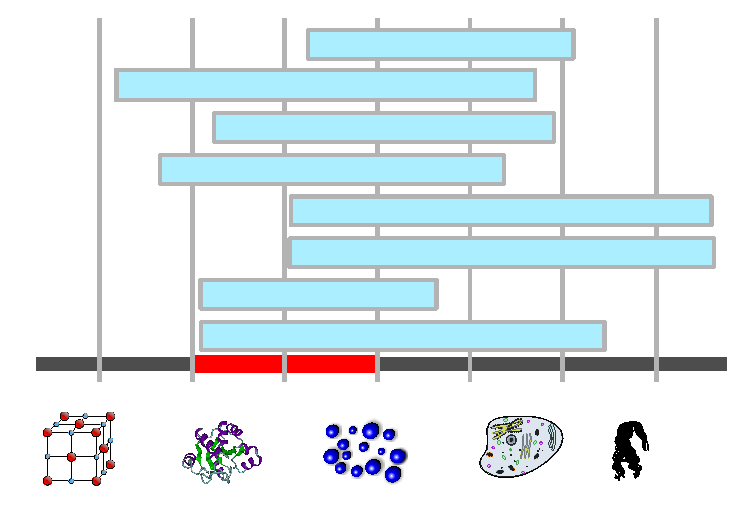
\includegraphics[width=0.95\textwidth]{Figures/SizeRange.pdf}
%		\caption[Sizing techniques]{Some available sizing techniques for nanoparticles and their available size range.}
%		\label{fig:SizeRange}
%\end{figure}

The nanoparticles envisioned for medical use tend to be found in the soft matter regime and thus the characterization tools must be carefully chosen considering the measurement limitations. For example, biodegradable NPs, e.g. polymeric colloids, are finding many medical applications, especially as drug-carriers \citep{kattan_phase_1992,vicent_polymer_2006} and are starting to undergo clinical trials \citep{patel_polymeric_2012,beija_colloidal_2012,cabral_progress_2014}. However, the size determination of polymeric NPs with a well-known technique like AFM is rather challenging \citep{wu_particle_2014} and suggests altenative approaches.

Liposomes are spheric vesicles composed of a closed phospholipid bilayer membrane capable of encapsulating hydrophilic compounds. The importance of lipid vesicles in the progress of nanomedicine is indisputable, as the first approved nanodrug is a liposomal formulation of doxorubicin, Doxil. Nowadays liposomes continue to be a widespread instrument for drug delivery \citep{perez-herrero_advanced_2015}, but their complicate internal structure requires typically more than a single a characterization tool \citep{khorasani_closing_2014}. Likewise, relevant biological structures in nanomedicine possess heterogenous morphologies rather difficult to detect with imaging techniques. For instance, electron microscopy is an effective tool for direct observation of the shape and size distribution of nanoparticles, but it cannot conclusively elucidate their inner composition.

The use of an ensemble-average and non-destructive technique such as small-angle X-ray scattering (SAXS) arises as an appropiate alternative \citep{leonard_jr_size_1952,motzkus_untersuchung_1959}. This technique can discern electron density differences in the structure of NPs and offers advantages to other methods which require prior treatment of the sample and are not averaging. SAXS is based on the elastic scattering of X-ray photons by the electron density distribution of an object and is traceable down to the SI unit \emph{nm} for the size determination of sufficiently monodisperse NPs \citep{meli_traceable_2012}. 

The first SAXS phenomena were observed in the 1930s by P. Krishnamurti and B.E. Warren \citep{krishnamurti_saxs_1930, warren_xray_1934} while investigating colloidal suspensions and carbon black systems. The instrumental advances introduced by O. Kratky and A. Guinier \citep{guinier_dispositif_1937,kratky_berechnung_1938} sparked the interest in the technique, while the seminal work of Guinier \citep{guinier_diffraction_1939} paved the way for the development of a SAXS theoretical background by scientists like Kratky, P. Debye or G. Porod \citep{kratky_bestimmung_1943,debye_scattering_1949,kratky_diffuse_1949,guinier_study_1950,guinier_small-angle_1955}. Stuhrmann's new approach to the understanding of the scattered intensity \citep{stuhrmann_elimination_1965} and the appearance of dedicated synchrotron radiation sources stimulated the scientific community to employ SAXS as a characterization tool. Since then, SAXS has been extensively employed in the characterization of polymeric colloids \citep{dingenouts_analysis_1999,chu_small-angle_2001,ballauff_analysis_2011} and its use in liposome research is also ubiquitous. For instance, it has been applied to characterize the lamellarity, bilayer thickness, area per lipid ratio \citep{pabst_applications_2010,bouwstra_small_1993,brzustowicz_x-ray_2005} and the thickness of the PEG-layer of different liposomal samples \citep{varga_closer_2010,varga_characterization_2012}, as well as to describe the influence of extrusion on the average number of bilayers \citep{jousma_characterization_1987} and to determine the electron density profile of liposomes \citep{bouwstra_small_1993,brzustowicz_x-ray_2005,hirai_determination_2003} and biological vesicles \citep{castorph_structure_2010}.

Despite being a highly informative method for the accurate characterization of NPs, the difficulties in the interpretation of the scattering curves in the reciprocal space demands complementary experimental information \citep{mykhaylyk_structural_2012}. The solvent contrast variation approach is a noteworthy candidate due to the complementary data that can be collected at each independent contrast. The contrast variation method in SAXS varies systematically the electron density of the suspending medium by adding a suitable contrast agent, e.g. sucrose, in order to resolve the different contributions of the particle components to the scattering. By measuring SAXS patterns as a function of the adjusted contrast, a more detailed insight into the particle morphology can be obtained in comparison to single-contrast experiments \citep{bolze_situ_2004}. For instance, the internal structure can be modelled in terms of the radial electron density \citep{dingenouts_radial_1994,dingenouts_analysis_1999,ballauff_analysis_2011,ballauff_small-angle_1996} and the individual contribution of each component can be distinguished \citep{beyer_saxs_1990,grunder_analysis_1991,grunder_small-angle_1993,ottewill_characterization_1995,bolze_small-angle_1997,dingenouts_structure_1994} as well as its density \citep{mykhaylyk_application_2007}.

This work proposes a novel approach to solvent contrast variation in SAXS based on the formation of a solvent density gradient within a capillary which enables the acquisition of SAXS patterns at a continuous range of contrasts and, as a result, collect in a relatively short timespan an extensive data set of complementary scattering curves. This intelligent strategy averts the most problematic issues of the classical solvent contrast variation technique, namely the discrete range of available solvent electron densities and the prolonged time required for the preparation of the complementary samples and for the obtention of the experimental data. Besides, the possibility to choose during the experiment the most appropriate contrast within the available range allows to tune \emph{in situ} the performance of the contrast variation technique in SAXS without \emph{a priori} knowledge of the investigated nanoparticles.

Following this introduction, chapter \ref{chap:theory_SAXS} is dedicated to describe the theoretical framework required to understand the contrast variation method in small-angle X-ray scattering. The instrumention employed for the obtention of the experimental results presented in this work is thoroughly described in chapter \ref{chap:experimental_setup}. These two chapters serve as the necessary building blocks for the development of the continuous contrast variation method based on the idea of a density gradient column. The detailed review of its performance is presented in chapter \ref{chap:density_gradient_SAXS}, where the technique is used to characterize low-density nanoparticles. The metrological possibilities of the newly introduced method are further evaluated in chapter \ref{chap:simultaneous_size_density}, focusing principally in its ability to determine the size and density of polymeric NPs in a traceable way. Finally, the scope of the technique is investigated in chapter \ref{chap:bio_applications} by using the continuous contrast variation method in a myriad of relevant nanomaterials related to nanomedicine or human biology. A last chapter \ref{chap:conclusions} acts as the necessary summary of the results presented in this work and comprises some conclusive remarks to this thesis. Extensive parts of the work presented in chapters \ref{chap:density_gradient_SAXS} to \ref{chap:bio_applications} have been published in peer-reviewed journals \citep{minelli_characterization_2014,garcia-diez_nanoparticle_2015,garcia-diez_size_2016,garcia-diez_simultaneous_2016-1}.

%The structure of this work feels organic, as depicted by the diagram in figure .



